\chapter{La question de la fiabilité des données}

On a donc vu que la donnée empruntait un chemin ardu, à travers plusieurs outils et sous plusieurs formes. Différentes équipes travaillent à différents moments sur ces données. Ces équipes ont des niveaux différents d’expertises de la donnée. Il est donc primordial de s’assurer de la fiabilité de ces données. Ainsi, il faut évaluer les performances des outils \Spider{} et \Arkindex{}, qui sont les principaux outils permettant à la donnée d’intégrer une base. Se pose également la question des serveurs, qui sont essentiels au projet, puisque l’ampleur des données collectées nécessite un endroit de stockage important, stable et accessible aux différentes équipes. On verra que conserver 100\% de l’intégralité des données est difficile dans un projet aussi complexe, aussi, il est intéressant d’anticiper la perte des données. 

    \section{Les performances des outils du projet, \Spider{} et \Arkindex{}}

Pour rappel, \Spider{} est l’outil qui permet d’associer les images numérisées par les services d’archives avec leurs métadonnées avant d’intégrer \Arkindex{}, la technologie HTR développée par Teklia. \Spider{} fait des erreurs, et il faut parfois relancer le processus plusieurs fois pour s’assurer que toutes les images sont traitées. Mais l’avantage est que l’outil prévient du nombre d’erreur. Dans ce cas, il faut explorer le fichier de métadonnées fourni par les services d’archives pour comprendre ce qui ne fonctionne pas. Cela ne requiert pas d’expertise particulière mais c’est réalisé par les équipes d’ingénieurs chez Teklia. 
C’est surtout lors du travail d’\Arkindex{} que la question de la fiabilité des données va se poser. Il faut cependant distinguer deux types de données. De fait, \Arkindex{} "double" la donnée : 

\begin{samepage}
\begin{itemize}
    \item On a toujours la donnée contenue dans les images numérisées
    \item On récupère la donnée créée à partir de ces images par le processus HTR
\end{itemize}
\end{samepage}
Il faut s’assurer de l’intégrité et donc de la fiabilité de ces deux types de données.\\

Concernant les images numérisées, c’est-à-dire les mots contenus dans les livres de recensement, on ne peut que faire confiance à ceux qui les ont rédigés, et accepter cette réalité telle quelle. Cependant, il y a un point à explorer : ces livres de recensement ont été aussi utilisés par les annotateurs pour nourrir et entraîner les modèles, comme \DAN{} ou \YOLO{} qui travailleront sur les images pour lire, reconnaître et extraire les données. Les annotateurs vont donc indexer, à la main, des listes de recensement : ils font le travail – manuellement – que les modèles seront amenés à faire par la suite de façon automatisée.  Les équipes d’annotateurs commencent par définir des zones\footnote{Extraits du mode d'emploi destiné aux annotateurs.} : 

\clearpage
\begin{figure}[H]
        \centering
        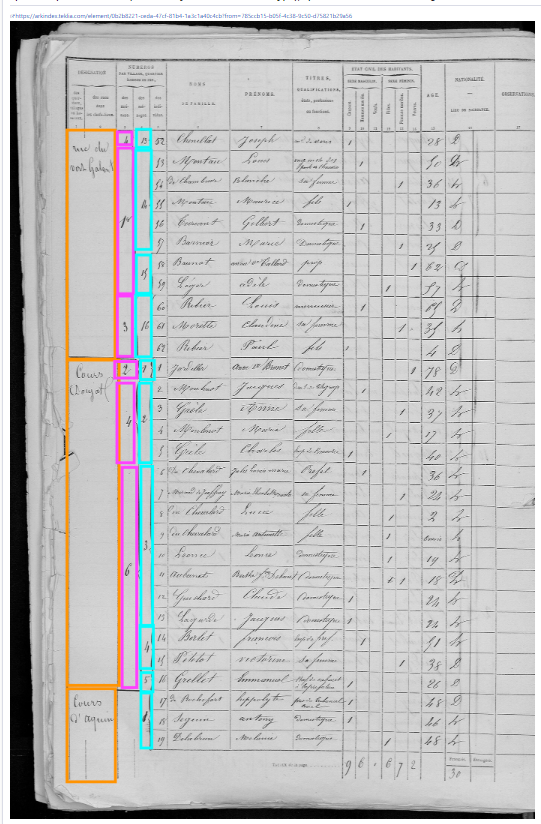
\includegraphics[width=0.8\linewidth]{Figures/Partie 2/Fig.2.4 - Exemple d'une page avec délimitation des zones - Mode d'emploi SocFace à destination des annotateurs.png}
        \caption[Exemple d'une page avec délimitation des zones]{Exemple d'une page avec délimitation des zones}
        \label{fig:Fig2.4}
    \end{figure}

Ceci n’est qu’un exemple, car les listes de recensement ont évolué dans leur format au fil du temps. C’est pourquoi il est primordial d’entraîner les modèles sur les différents types de listes que l’on peut trouver.\\ 
\clearpage
La deuxième étape, c’est l’indexation des mentions. On le voit, l’écriture n’est pas toujours simple à déchiffrer et dans certains cas, le scripteur a utilisé une abréviation. 
\begin{figure}[H]
        \centering
        \includegraphics[width=0.95\linewidth]{Figures/Partie 2/Fig.2.5 - Exemple des champs à remplir pour l'annotation.png}
        \caption{Exemple des champs à remplir pour l'annotation}
        \label{fig:Fig2.5}
    \end{figure}

Ainsi, une partie du traitement est manuelle, et un humain est plus susceptible de faire une erreur qu’une machine, même si on verra que les machines en font aussi. En effet, lorsque les modèles travaillent sur la lecture des données, on voit qu’elles peuvent avoir ce qu’on appelle des hallucinations : cette technologie est prédictive, elle utilise les informations qu’on lui a fourni pour prédire à son tour la nature des mentions qu’elle lit. Mais ces technologies basées sur le \gls{DL} ne peuvent pas admettre quand elles ne savent pas ou quand elles doutent. Dès lors, elles vont « reconnaître » un mot ou une date qui n’est pas la bonne. On dit qu’elles ont des hallucinations. Ou bien ne pas voir qu’il s’agit de deux pages différentes ou qu'une page se termine. Cela peut s’expliquer par une mauvaise numérisation, avec un contraste faible, ou bien une mauvaise qualité de la source elle-même (bien que les listes de recensement soient dans l’ensemble bien conservées). Il peut également avoir des problèmes au moment de l’export \Arkindex{} vers Teklia. L’HTR se comporte correctement mais au moment de l’export, des lignes sont manquantes ou des mentions n’existent plus.\\
SocFace est un projet complexe et multidisciplinaire. Le type d’erreur découle de la technologie utilisée, mais également du fait que le chemin de la donnée emprunte différent support. La base de données finale est le résultat conjoint de la technologie, mise au point par des ingénieurs informatiques de Teklia, des annotations faites par des annotateurs recrutés et l’analyse des chercheurs de l’INED. C’est le fruit d’une interdisciplinarité et d’une collaboration entre différents acteurs. C’est une nécessité pour le projet, mais c’est également l’une des raisons pour lesquelles ces erreurs peuvent arriver. La donnée est produite par la conjonction de plusieurs expertises, mais au prix d’un processus long et dont les étapes sont opérées par des acteurs différents. Encore une fois, on voit que l’interdisciplinarité est nécessaire, mais également à l’origine de questionnements sur le projet, en l’espèce sur la fiabilité même des données. 

    \section{Plusieurs serveurs pour une donnée fiable}

La question des serveurs est bien évidemment primordiale pour gérer la pérennité des données.  Ces serveurs jouent deux rôles :
\begin{itemize}[label=\textbullet]
    \item Ils apportent \textbf{la puissance de calcul} pour le processus de lecture et d’extraction des données
    \item Ils permettent \textbf{le stockage des données}, que ce soit les images numérisées, puis la base de données elle-même.
\end{itemize}

Concernant la puissance de calcul, elle est nécessaire pour mener à bien le processus. En l’espèce, vu le nombre considérable de pages à traiter et de données à extraire, il est nécessaire de s’appuyer sur un supercalculateur. SocFace utilise donc Jean Zay, qui appartient et est maintenu par le CNRS. Pour avoir le droit d'utiliser ce serveur, qui est un des plus puissants d'Europe\footnote{\href{https://www.top500.org/lists/top500/list/2024/06/?page=4}{https://www.top500.org/lists/top500/list/2024/06/?page=4}}, il faut démontrer un projet de recherche, non commercial, et d'une expertise suffisante des membres de l'équipe. Ici, SocFace a demandé 200 000 heures d'utilisation.
Cette puissance de calcul est d’autant plus nécessaire pour SocFace que comme on l’a vu, \Arkindex{} effectue l’ensemble des opérations de reconnaissance du texte manuscrit en un seul passage, contrairement à ce qui se fait en principe dans ce genre de projet. C’est un modèle intégré. Or, plus le serveur est puissant, plus les résultats sont solides : cela limite le nombre d’erreurs, ou d’hallucinations possibles. Il fallait donc pour SocFace un supercalculateur. Si Jean Zay est nécessaire, il est aussi instable. Le projet est tributaire de la maintenance par le CNRS, des mises à jour, et des nombreuses autres utilisations qui sont faites du supercalculateur. Cette collaboration est nécessaire, mais est à l’origine de certains ralentissements et nécessite aux équipes du projet de s’adapter.\\
Concernant les serveurs pour le stockage des données, ils sont plus nombreux. Comme on l’a vu, Teklia a ses propres serveurs, et ils sont utilisés pour stocker les images numérisées avant l’intégration des données, puis lors du traitement sur \Arkindex{}. Mais par la suite, la base de données est hébergée par un serveur de l’INED. Elle est répliquée sur un serveur de Teklia, et à terme, le SIAF aura également sa propre base de données sur ses propres serveurs. Cela fait donc trois serveurs pour trois bases de données, qui ne doivent pas être dissociées, car il faut s’assurer de l’adéquation des bases de données entre elles. A ce jour, la base de données du SIAF n’existe pas (comme on l’a vu, ils travaillent pour l’instant sur un dump), on ne peut donc pas présager d’une dissociation ou d’une perte des données. Concernant Teklia et l’INED, c’est une réplication, avec une synchronisation en temps réel, pour empêcher ce genre de problèmes. Cette connexion peut poser des problèmes. En effet l’INED est une institution publique. 
\\A ce titre, il y a certaines contraintes : 

\begin{itemize}
    \item Respect des protocoles de sécurité, pour protéger le réseau
    \item On ne peut pas permettre l’accès au serveur à n’importe qui, il faut donc privilégier les ingénieurs qui travailleront dessus
    \item Le serveur de l’INED est partagé avec tous les autres équipes de recherches de l’INED, SocFace ne peut donc pas agir à sa guise et doit passer par les équipes IT de l’INED.
\end{itemize}

Par exemple, utiliser Metabase ailleurs qu’à l’INED s’est révélé impossible car le programme est connecté au serveur de l’INED. Jongler entre ces différents serveurs nécessite une bonne communication entre les équipes qui collaborent. Il faut s’adapter constamment pour trouver des solutions, là où dans un projet mené par un seul acteur ou dans une seule discipline, la question se serait moins posée car ils auraient pu disposer de leur propre serveur. Et dans le même temps, ce type de projet n’aurait sûrement pas eu la même envergure et n’aurait pas eu besoin d’autant de puissance et de stockage. \\
On voit donc que les outils et les serveurs utilisés pour le projet, s’ils sont nécessaires et pensés pour traiter des données de grande ampleur, ne sont pas à l’abri de provoquer des erreurs dans l’écriture des données. Comment dès lors anticiper ce qui peut amener à une perte des données ou à leur dégradation ?


    \section{Comment palier la perte des données?}

Les équipes de SocFace doivent composer avec la possibilité d’erreurs dans les données, que ce soit dans l’indexation, dans le transfert ou dans l’écriture de la donnée. Comment anticiper cela ? Quel seuil d’erreur est acceptable ? Comment régler les erreurs une fois qu’elles sont repérées.\\ 

On l’a vu, les erreurs peuvent intervenir dès l’entraînement des modèles par les annotateurs qui utilisent le système Callico. Pour limiter au maximum les erreurs humaines, SocFace a produit de la documentation avec des consignes à suivre\footnote{Voir Annexe G} . Cela permet également d’assurer une certaine cohérence dans les données. Par exemple, conserver les accents, développer les abréviations, corriger les fautes d’orthographe évidentes etc… Il faut aussi comprendre que les difficultés ne sont pas les mêmes selon le type de mention : il est plus facile de se tromper sur un nom de famille peu courant que sur une année où les combinaisons différentes sont beaucoup moins nombreuses que pour un mot. Cela permet également de normaliser les mentions. Par exemple, s’assurer que la mention "cultivateur", souvent abrégée en "culti", soit bien développée. 
Pour autant, malgré l’encadrement des annotateurs, il peut y avoir des erreurs. C’est le cas pour la mention "idem" ou "id.". Cette mention est très utilisée par le scripteur, pour simplifier son travail. On la trouve notamment dans la colonne « nationalité » ou pour le nom de famille d’un même foyer. Certains annotateurs ont développé le "idem" en réécrivant la mention. Il a donc fallu développer un programme pour récupérer la mention "idem" à la place de la réécriture de l’annotateur. Ce type de correction manuelle sont faites à posteriori, une fois que les erreurs ont été détectées. On peut l’utiliser pour d’autres types d’erreurs qui ont été repérées ou pour favoriser la normalisation. Par exemple retirer le "ans" lorsque l’âge est mentionné.\\
Ces erreurs sont donc détectées après l’écriture des données dans une procédure de "nettoyage". Les chercheurs de l’INED qui ont accès à la base de données navigue à travers les données déjà produites afin de voir les incohérences qui peuvent ressortir. Au vu de l’ampleur des données, il est bien entendu impossible de faire une vérification précise. Par exemple, une des expériences tentée a été de comparer le nombre de mention de nom par commune – c’est-à-dire le nombre d’habitant – avec les chiffres de l’INSEE sur les mêmes années. Si les chiffres divergent trop, cela signifie certainement qu’il manque des pages sur la commune ou bien qu’il y a eu un doublement de l’export des données. Ces tests sont effectués majoritairement par les chercheurs de l’INED. Dans tous les cas, il faut avoir un accès à la base de données pour cela, et ce n’est pas le cas de tous les membres de l’équipe. Mais cela reste un bon exemple de collaboration interdisciplinaire : un développeur peut créer un script de correction de données en se basant sur les analyses faites par un démographe.\\

On voit donc que des moyens sont mis en place pour limiter les possibilités d’erreurs. Soit par anticipation, soit par correction, une fois les erreurs détectées. Mais dans les deux cas, il faut accepter un taux d’erreur possible. On parle de la numérisation de près de 15 millions de pages et donc l’écriture de plusieurs centaines de millions de mentions. Il faut donc déterminer un seuil d’erreur acceptable, qui devra être pris en compte par les chercheurs dans leur réutilisation de la donnée.

Ce chapitre a permis de souligner l’importance de la gestion des données dans le projet SocFace. La nature complexe et diversifiée des données, ainsi que les multiples acteurs impliqués imposent des défis techniques et juridiques significatifs. En détaillant les processus de collecte, d’intégration, de visualisation et de sécurisation des données, nous avons montré comment ces éléments se conjuguent pour transformer des informations brutes en une base de connaissances structurée, apte à soutenir des recherches futures. L’interdisciplinarité, au cœur du projet, exige une collaboration étroite et une harmonisation continue des efforts pour maintenir l’intégrité et la cohérence des données, tout en respectant les cadres légaux en vigueur. Après avoir vu ces considérations techniques et organisationnelles, nous allons explorer plus en détail les perspectives offertes par l’analyse de ces données : les méthodologies employées pour extraire des connaissances pertinentes des vastes ensembles de données accumulées, ainsi que les enjeux liés à l’exploitation de ces données dans un cadre de recherche. 